\documentclass[a4paper,11pt]{article}
\usepackage[utf8]{inputenc}
\usepackage[spanish]{babel}
\usepackage[affil-it]{authblk}
\usepackage{enumerate}
\usepackage{graphicx}
\usepackage{hyperref}
\usepackage{amsmath}
\usepackage{amssymb}
\usepackage{cancel}
\usepackage[usenames, dvipsnames]{color}
\usepackage{tikz}
\usepackage[labelfont=bf]{caption}
\usepackage{subcaption} %Multiple images
\usepackage{multicol} % Multiple columns
\usepackage{float}
\usepackage{cleveref}
\usepackage{relsize} % bigger math symbols
\usepackage[margin=1.1in]{geometry}
\usepackage[titletoc,toc,title]{appendix}
\usepackage{enumitem}
\usepackage{etoolbox}
\usepackage{mdframed} %frame theorems
\usetikzlibrary{calc}
\numberwithin{equation}{section}

% Footnotes with symbols

\makeatletter
\def\@fnsymbol#1{\ensuremath{\ifcase#1\or \dagger\or \ddagger\or
   \mathsection\or \mathparagraph\or \|\or **\or \dagger\dagger
   \or \ddagger\ddagger \else\@ctrerr\fi}}
\makeatother

\renewcommand{\thefootnote}{\fnsymbol{footnote}}

% Cool letters 
%Filename:      Typocaps.fd
%Created by:    MLO
%Creation date: 2003/04/02

% This file should be put in a TeX input directory

\ProvidesFile{Typocaps.fd}
   [2003/04/02 Font definition file for U/Typocaps]

\DeclareFontFamily{U}{Typocaps}{}

\DeclareFontShape{U}{Typocaps}{xl}{n}{
   <-> Typocaps
}{}

\endinput


% Footer
\usepackage{fancyhdr}
\pagestyle{fancy}
\fancyhf{}
\cfoot{\fontsize{15pt}{15pt}\usefont{U}{Typocaps}{xl}{n} 
gigantium humeris insidentes}

% Big Pictures
\usepackage[export]{adjustbox}

% Enviroment for theorems
\newmdtheoremenv[frametitle=Teorema]{theo}{Theorem}

% Circled words
\newcommand{\circled}[2][]{%
  \tikz[baseline=(char.base)]{%
    \node[shape = circle, draw, inner sep = 1pt]
    (char) {\phantom{\ifblank{#1}{#2}{#1}}};%
    \node at (char.center) {\makebox[0pt][c]{#2}};}}
\robustify{\circled}

%Appendices in spanish
\renewcommand{\appendixname}{Ap\'endices}
\renewcommand{\appendixtocname}{Ap\'endices}
\renewcommand{\appendixpagename}{Ap\'endices}

%Zero delimiter
\newcommand{\zerodel}{.\kern-\nulldelimiterspace}

%Columns separation
\setlength{\columnsep}{1cm}

%Indentation
\setlength{\parindent}{0ex}

%Multiple References

\crefrangelabelformat{equation}{(#3#1#4--#5\crefstripprefix{#1}{#2}#6)}

\usepackage{xparse}

%Boxes

\newcommand*{\boxcolor}{blue}
\makeatletter
\renewcommand{\boxed}[1]{\textcolor{\boxcolor}{%
\tikz[baseline={([yshift=-1ex]current bounding box.center)}] \node [rectangle, minimum width=1ex,rounded corners,draw] {\normalcolor\m@th$\displaystyle#1$};}}
 \makeatother

%Constantes
\newcommand{\euler}{\mathrm{e}}
\newcommand{\im}{i}

%Lemas, teoremas, definiciones y pruebas
\newcommand{\definicion}{\textbf{Definición: }}
\newcommand{\lema}{\textbf{Lema: }}
\newcommand{\teorema}{\textbf{Teorema: }}
\newcommand{\prueba}{\textbf{Prueba: }}
\newcommand{\proposicion}{\textbf{Proposición: }}
\newcommand{\corolario}{\textbf{Corolario: }}

% Definición de las secciones y su numeración

\makeatletter
\def\@seccntformat#1{%
  \expandafter\ifx\csname c@#1\endcsname\c@section\else
  \csname the#1\endcsname\quad
  \fi}
\makeatother

\begin{document}

\begin{titlepage}
\thispagestyle{fancy}

\newcommand{\HRule}{\rule{\linewidth}{0.5mm}} % Defines a new command for the horizontal lines, change thickness here

\center % Center everything on the page
 
%----------------------------------------------------------------------------------------
%	HEADING SECTIONS
%----------------------------------------------------------------------------------------

\textsc{\LARGE Universidad Nacional Autónoma de México}\\[0.3cm] % Name of your university/college

%----------------------------------------------------------------------------------------
%	LOGO SECTION
%----------------------------------------------------------------------------------------


\includegraphics[scale=0.17]{unam}

%----------------------------------------------------------------------------------------
%	SUBHEADING SECTIONS
%----------------------------------------------------------------------------------------

\textsc{\Large Electrodinámica Clásica}\\[0.3cm] % Major heading such as course name
\textsc{\large Semestre 2016-II}\\[0.3cm] % Minor heading such as course title
\textsc{\large 17 de marzo de 2016}\\ % Minor heading such as course title

%----------------------------------------------------------------------------------------
%	TITLE SECTION
%----------------------------------------------------------------------------------------

\HRule \\[0.1cm]
{ \huge \bfseries Tarea \# 5. \\ Ecuaciones de Maxwell, 
electromagnetismo macroscópico y leyes de conservación.}\\ % Title of your document
\HRule \\[0.1cm]
 
%----------------------------------------------------------------------------------------
%	AUTHOR SECTION
%----------------------------------------------------------------------------------------
\setcounter{footnote}{0}
\center
\large
\emph{Autor:} \\ % Your name
\Large Favio \textsc{Vázquez}\footnote[1]{\href{mailto:favio.vazquez@correo.nucleares.unam.mx}{favio.vazquez@correo.nucleares.unam.mx}}
\\[0.7cm]
%----------------------------------------------------------------------------------------
%	COOL IMAGE SECTION
%----------------------------------------------------------------------------------------

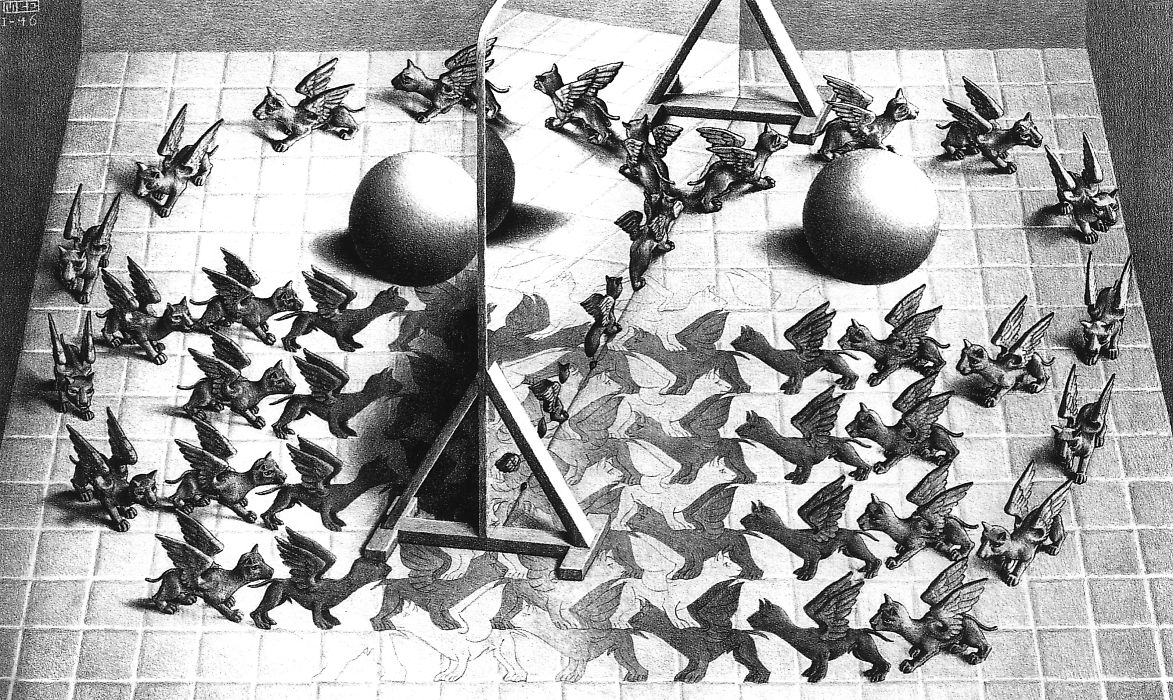
\includegraphics[scale=1.55]{escherEspejo2D}

%----------------------------------------------------------------------------------------

\vfill % Fill the rest of the page with whitespace

\end{titlepage}

% ---------------------------------------------------------------------------------------
%         HEADER
%----------------------------------------------------------------------------------------

\fancyhead[L]{Favio Vázquez}
\fancyhead[R]{\thepage}

%----------------------------------------------------------------------------------------
\setcounter{footnote}{0}
\renewcommand*{\thefootnote}{\arabic{footnote}}
%----------------------------------------------------------------------------------------

%----------------------------------------------------------------------------------------
%%			BEGIN DOCUMENT
%----------------------------------------------------------------------------------------

\section{Problema 1. Problema 6.8 de Classical Electromagnetic Radiation
de Jackson \cite{jackson}.}

Una esfera de constante dieléctrica constante $\epsilon$ y radio $a$ está situada 
en el origen. Hay un campo eléctrico $E_0$ uniforme aplicado en la dirección $x$. 
La esfera rota con una velocidad angular $\omega$ sobre el eje $z$. Muestre que 
hay un campo magnético $\mathbf{H} = - \mathbf{\nabla} \Phi_M$, donde 

$$
\Phi_M = \frac{3}{5}\left(\frac{\epsilon - \epsilon_0}{\epsilon + 2\epsilon_0}\right)
\epsilon_0E_0\omega\left(\frac{a}{r_>}\right)\cdot xz,
$$

donde $r_>$ es el más grande de $r$ y $a$. El movimiento es no relativista. Puede 
utilizar los resultados de la sección $4.4$ para la esfera dieléctrica en un campo 
aplicado.

\vspace{.3cm}

\underline{Solución:} \vspace{.3cm}

\newpage

\section{Problema 2. Problema 6.9 de Classical Electromagnetic Radiation
de Jackson \cite{jackson}.}

Discuta la conservación de la energía y el impulso lineal para un sistema macroscópico 
de fuentes y campos electromagnéticos en un medio uniforme e isotrópico, descrito 
por una permitividad $\epsilon$ y una permeabilidad $\mu$. Muestre en un cálculo 
simple que la densidad de energía, el vector de Poynting, la densidad de campo-impulso, 
y el tensor de esfuerzo de Maxwell están dados por las expresiones de Minkowski,

\begin{align*}
u &= \frac{1}{2}(\epsilon E^2 + \mu H^2), \\
\mathbf{S} &= \mathbf{E} \times \mathbf{H}, \\
\mathbf{g} &= \mu\epsilon \mathbf{E} \times \mathbf{H}, \\
T_{ij} &= [\epsilon E_iE_j + \mu H_iH_j - \frac{1}{2}\delta_{ij}(\epsilon E^2 + \mu H^2)].
\end{align*}

¿Qué modificaciones surgen si $\epsilon$ y $\mu$ son funciones de la posición?

\vspace{.3cm}

\underline{Solución:} \vspace{.3cm}

\newpage

\section{Problema 3. Problema 6.15 de Classical Electromagnetic Radiation
de Jackson \cite{jackson}.}

Un capacitor de placas paralelas circular ideal de radio $a$ y separación entre 
las placas $d \ll a$ está conectado a una fuente de corriente mediante hilos de 
conexión axial, como se muestra en el bosquejo. La corriente en el cable es 
$I(t) = I_0\cos{\omega t}$.

\begin{figure}[H]
 \center 
 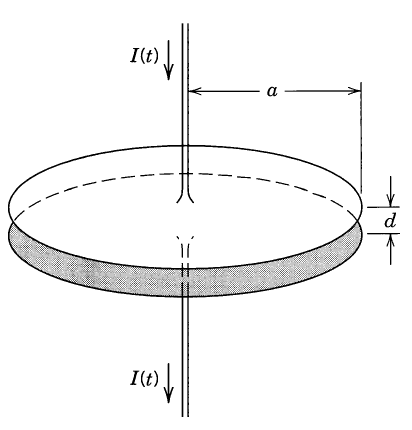
\includegraphics[scale=0.5]{problema3fig1}
\end{figure}

\begin{enumerate}[label=\textbf{(\alph*)}]
\item Calcule el campo eléctrico y el magnético entre las placas a segundo orden 
en potencias de la frecuencia (o número de onda), despreciado los efectos de campos 
de borde.
\item Calcule las integrales de volumen de $w_e$ y $w_m$ que entran en la definición 
de la reactancia $X$, (6.140), a segundo orden en $\omega$. Muestre que en términos 
de la corriente de entrada $I_i$, definida por $I_i = - i\omega Q$, donde $Q$ es 
a la carga total en una placa, estas energías son 

$$
\int w_e d^3 = \frac{1}{4\pi\epsilon}\frac{|I_i|^2d}{\omega^2 a^2}, \qquad 
\int w_m d^3 = \frac{\mu_0}{4\pi}\frac{|I_i|^2d}{8}\left(1 +
\frac{\omega^2 a^2}{12c^2} \right).
$$
\item Muestre que los circuitos en serie equivalentes tienen $C \simeq \pi\epsilon_0 
a^2/d$, $L \simeq \mu_0d/8\pi$, y que un estimado para la frecuencia de resonancia 
del sistema es $\omega_{res} \simeq 2\sqrt{2}c/a$. Compare con la primera raíz 
de $J_0(x)$.
\end{enumerate}

\vspace{.3cm}

\underline{Solución:} \vspace{.3cm}

\newpage

\begin{thebibliography}{10}
\bibitem{jackson}
J. Jackson, \emph{Classical Electrodynamics}, 3ra edición. John Wiley and Sons, Inc. 
1999.
\end{thebibliography}

\end{document}